\documentclass{standalone}
\usepackage{tikz}
\usetikzlibrary{patterns, positioning}


\begin{document}
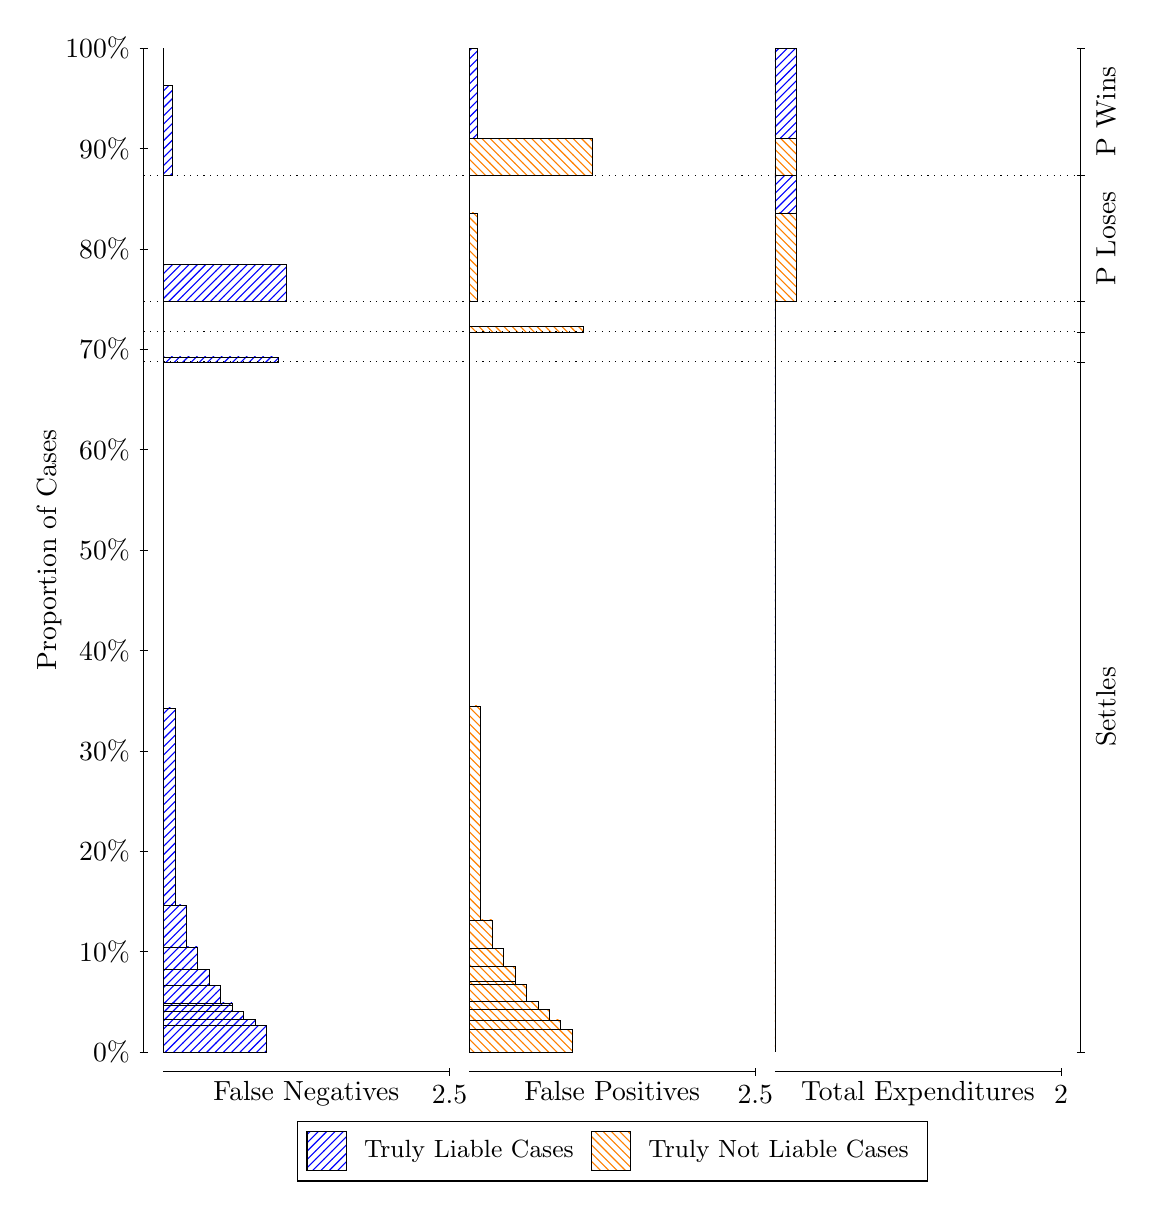
\begin{tikzpicture}
\draw[black, very thin] (1.5,1.75) -- (1.5,14.5);
\node[rotate=90, text=black, anchor=center] at (0.3, 8.125) {Proportion of Cases};
\draw[black, very thin] (1.45,1.75) -- (1.55,1.75);
\node[text=black, anchor=east] at (1.45, 1.75) {0\%};
\draw[black, very thin] (1.45,3.025) -- (1.55,3.025);
\node[text=black, anchor=east] at (1.45, 3.025) {10\%};
\draw[black, very thin] (1.45,4.3) -- (1.55,4.3);
\node[text=black, anchor=east] at (1.45, 4.3) {20\%};
\draw[black, very thin] (1.45,5.575) -- (1.55,5.575);
\node[text=black, anchor=east] at (1.45, 5.575) {30\%};
\draw[black, very thin] (1.45,6.85) -- (1.55,6.85);
\node[text=black, anchor=east] at (1.45, 6.85) {40\%};
\draw[black, very thin] (1.45,8.125) -- (1.55,8.125);
\node[text=black, anchor=east] at (1.45, 8.125) {50\%};
\draw[black, very thin] (1.45,9.4) -- (1.55,9.4);
\node[text=black, anchor=east] at (1.45, 9.4) {60\%};
\draw[black, very thin] (1.45,10.675) -- (1.55,10.675);
\node[text=black, anchor=east] at (1.45, 10.675) {70\%};
\draw[black, very thin] (1.45,11.95) -- (1.55,11.95);
\node[text=black, anchor=east] at (1.45, 11.95) {80\%};
\draw[black, very thin] (1.45,13.225) -- (1.55,13.225);
\node[text=black, anchor=east] at (1.45, 13.225) {90\%};
\draw[black, very thin] (1.45,14.5) -- (1.55,14.5);
\node[text=black, anchor=east] at (1.45, 14.5) {100\%};

\draw[black, very thin] (13.4,1.75) -- (13.4,14.5);
\draw[black, very thin] (13.35,1.75) -- (13.45,1.75);
\node[anchor=west] at (13.35, 1.75) {};
\draw[black, very thin] (13.35,10.514) -- (13.45,10.514);
\node[anchor=west] at (13.35, 10.514) {};
\draw[black, very thin] (13.35,10.896) -- (13.45,10.896);
\node[anchor=west] at (13.35, 10.896) {};
\draw[black, very thin] (13.35,11.283) -- (13.45,11.283);
\node[anchor=west] at (13.35, 11.283) {};
\draw[black, very thin] (13.35,12.881) -- (13.45,12.881);
\node[anchor=west] at (13.35, 12.881) {};
\draw[black, very thin] (13.35,14.5) -- (13.45,14.5);
\node[anchor=west] at (13.35, 14.5) {};

\draw[black, very thin, pattern color=blue, pattern=north east lines] (1.75,1.75) rectangle (3.058,2.0844);
\draw[black, very thin, pattern color=blue, pattern=north east lines] (1.75,2.0844) rectangle (2.9127,2.1679);
\draw[black, very thin, pattern color=blue, pattern=north east lines] (1.75,2.1679) rectangle (2.7673,2.2682);
\draw[black, very thin, pattern color=blue, pattern=north east lines] (1.75,2.2682) rectangle (2.622,2.3381);
\draw[black, very thin, pattern color=blue, pattern=north east lines] (1.75,2.3381) rectangle (2.622,2.3736);
\draw[black, very thin, pattern color=blue, pattern=north east lines] (1.75,2.3736) rectangle (2.4767,2.593);
\draw[black, very thin, pattern color=blue, pattern=north east lines] (1.75,2.593) rectangle (2.3313,2.7953);
\draw[black, very thin, pattern color=blue, pattern=north east lines] (1.75,2.7953) rectangle (2.186,3.086);
\draw[black, very thin, pattern color=blue, pattern=north east lines] (1.75,3.086) rectangle (2.0407,3.6187);
\draw[black, very thin, pattern color=blue, pattern=north east lines] (1.75,3.6187) rectangle (1.8953,6.1196);
\draw[black, very thin, pattern color=orange, pattern=north west lines] (1.75,6.1196) rectangle (1.75,10.514);
\draw[black, very thin, pattern color=blue, pattern=north east lines] (1.75,10.514) rectangle (3.2033,10.578);
\draw[black, very thin, pattern color=orange, pattern=north west lines] (1.75,10.578) rectangle (1.75,10.896);
\draw[black, very thin, pattern color=orange, pattern=north west lines] (1.75,10.896) rectangle (1.75,10.96);
\draw[black, very thin, pattern color=blue, pattern=north east lines] (1.75,10.96) rectangle (1.75,11.283);
\draw[black, very thin, pattern color=blue, pattern=north east lines] (1.75,11.283) rectangle (3.3123,11.757);
\draw[black, very thin, pattern color=orange, pattern=north west lines] (1.75,11.757) rectangle (1.75,12.881);
\draw[black, very thin, pattern color=blue, pattern=north east lines] (1.75,12.881) rectangle (1.859,14.026);
\draw[black, very thin, pattern color=orange, pattern=north west lines] (1.75,14.026) rectangle (1.75,14.5);
\draw[black, very thin, pattern color=orange, pattern=north west lines] (5.6333,1.75) rectangle (6.9413,2.04);
\draw[black, very thin, pattern color=orange, pattern=north west lines] (5.6333,2.04) rectangle (6.796,2.1583);
\draw[black, very thin, pattern color=orange, pattern=north west lines] (5.6333,2.1583) rectangle (6.6507,2.2903);
\draw[black, very thin, pattern color=orange, pattern=north west lines] (5.6333,2.2903) rectangle (6.5053,2.3935);
\draw[black, very thin, pattern color=orange, pattern=north west lines] (5.6333,2.3935) rectangle (6.36,2.6114);
\draw[black, very thin, pattern color=orange, pattern=north west lines] (5.6333,2.6114) rectangle (6.2147,2.6495);
\draw[black, very thin, pattern color=orange, pattern=north west lines] (5.6333,2.6495) rectangle (6.2147,2.8362);
\draw[black, very thin, pattern color=orange, pattern=north west lines] (5.6333,2.8362) rectangle (6.0693,3.064);
\draw[black, very thin, pattern color=orange, pattern=north west lines] (5.6333,3.064) rectangle (5.924,3.4276);
\draw[black, very thin, pattern color=orange, pattern=north west lines] (5.6333,3.4276) rectangle (5.7787,6.1446);
\draw[black, very thin, pattern color=blue, pattern=north east lines] (5.6333,6.1446) rectangle (5.6333,10.514);
\draw[black, very thin, pattern color=orange, pattern=north west lines] (5.6333,10.514) rectangle (5.6333,10.832);
\draw[black, very thin, pattern color=blue, pattern=north east lines] (5.6333,10.832) rectangle (5.6333,10.896);
\draw[black, very thin, pattern color=orange, pattern=north west lines] (5.6333,10.896) rectangle (7.0867,10.96);
\draw[black, very thin, pattern color=blue, pattern=north east lines] (5.6333,10.96) rectangle (5.6333,11.283);
\draw[black, very thin, pattern color=orange, pattern=north west lines] (5.6333,11.283) rectangle (5.7423,12.407);
\draw[black, very thin, pattern color=blue, pattern=north east lines] (5.6333,12.407) rectangle (5.6333,12.881);
\draw[black, very thin, pattern color=orange, pattern=north west lines] (5.6333,12.881) rectangle (7.1957,13.355);
\draw[black, very thin, pattern color=blue, pattern=north east lines] (5.6333,13.355) rectangle (5.7423,14.5);
\draw[black, very thin, pattern color=orange, pattern=north west lines] (9.5167,1.75) rectangle (9.5167,6.1446);
\draw[black, very thin, pattern color=blue, pattern=north east lines] (9.5167,6.1446) rectangle (9.5167,10.514);
\draw[black, very thin, pattern color=orange, pattern=north west lines] (9.5167,10.514) rectangle (9.5167,10.832);
\draw[black, very thin, pattern color=blue, pattern=north east lines] (9.5167,10.832) rectangle (9.5167,10.896);
\draw[black, very thin, pattern color=orange, pattern=north west lines] (9.5167,10.896) rectangle (9.5167,10.96);
\draw[black, very thin, pattern color=blue, pattern=north east lines] (9.5167,10.96) rectangle (9.5167,11.283);
\draw[black, very thin, pattern color=orange, pattern=north west lines] (9.5167,11.283) rectangle (9.7892,12.407);
\draw[black, very thin, pattern color=blue, pattern=north east lines] (9.5167,12.407) rectangle (9.7892,12.881);
\draw[black, very thin, pattern color=orange, pattern=north west lines] (9.5167,12.881) rectangle (9.7892,13.355);
\draw[black, very thin, pattern color=blue, pattern=north east lines] (9.5167,13.355) rectangle (9.7892,14.5);
\draw[black, dotted] (1.5,10.514) -- (13.4,10.514);
\draw[black, dotted] (1.5,10.896) -- (13.4,10.896);
\draw[black, dotted] (1.5,11.283) -- (13.4,11.283);
\draw[black, dotted] (1.5,12.881) -- (13.4,12.881);
\draw[black, very thin] (1.75,1.5) -- (5.3833,1.5);
\node[text=black, anchor=north] at (3.5667, 1.5) {False Negatives};
\draw[black, very thin] (5.3833,1.45) -- (5.3833,1.55);
\node[text=black, anchor=north] at (5.3833, 1.45) {2.5};

\draw[black, very thin] (5.6333,1.5) -- (9.2667,1.5);
\node[text=black, anchor=north] at (7.45, 1.5) {False Positives};
\draw[black, very thin] (9.2667,1.45) -- (9.2667,1.55);
\node[text=black, anchor=north] at (9.2667, 1.45) {2.5};

\draw[black, very thin] (9.5167,1.5) -- (13.15,1.5);
\node[text=black, anchor=north] at (11.333, 1.5) {Total Expenditures};
\draw[black, very thin] (13.15,1.45) -- (13.15,1.55);
\node[text=black, anchor=north] at (13.15, 1.45) {2};

\node[text=black, centered, rotate=90] at (13.72, 6.1321) {Settles};


\node[text=black, centered, rotate=90] at (13.72, 12.082) {P Loses};
\node[text=black, centered, rotate=90] at (13.72, 13.691) {P Wins};

\draw (7.449999999999999,1.5) node[draw=none] (baseCoordinate) {};
\begin{scope}[align=center]
        \matrix[scale=0.5, draw=black, below=0.5cm of baseCoordinate, nodes={draw}, column sep=0.1cm]{
            \node[rectangle, draw, minimum width=0.5cm, minimum height=0.5cm, pattern color=blue, pattern=north east lines] {}; &
            \node[draw=none, font=\small, text=black] (B) {Truly Liable Cases}; &
            \node[rectangle, draw, minimum width=0.5cm, minimum height=0.5cm, pattern color=orange, pattern=north west lines] {}; &
            \node[draw=none, font=\small, text=black] (B) {Truly Not Liable Cases}; \\
            };
\end{scope}

\end{tikzpicture}
\end{document}